\documentclass[]{book}
\usepackage{lmodern}
\usepackage{amssymb,amsmath}
\usepackage{ifxetex,ifluatex}
\usepackage{fixltx2e} % provides \textsubscript
\ifnum 0\ifxetex 1\fi\ifluatex 1\fi=0 % if pdftex
  \usepackage[T1]{fontenc}
  \usepackage[utf8]{inputenc}
\else % if luatex or xelatex
  \ifxetex
    \usepackage{mathspec}
  \else
    \usepackage{fontspec}
  \fi
  \defaultfontfeatures{Ligatures=TeX,Scale=MatchLowercase}
\fi
% use upquote if available, for straight quotes in verbatim environments
\IfFileExists{upquote.sty}{\usepackage{upquote}}{}
% use microtype if available
\IfFileExists{microtype.sty}{%
\usepackage{microtype}
\UseMicrotypeSet[protrusion]{basicmath} % disable protrusion for tt fonts
}{}
\usepackage[margin=1in]{geometry}
\usepackage{hyperref}
\hypersetup{unicode=true,
            pdftitle={A Minimal Book Example},
            pdfauthor={Yihui Xie},
            pdfborder={0 0 0},
            breaklinks=true}
\urlstyle{same}  % don't use monospace font for urls
\usepackage{natbib}
\bibliographystyle{apalike}
\usepackage{color}
\usepackage{fancyvrb}
\newcommand{\VerbBar}{|}
\newcommand{\VERB}{\Verb[commandchars=\\\{\}]}
\DefineVerbatimEnvironment{Highlighting}{Verbatim}{commandchars=\\\{\}}
% Add ',fontsize=\small' for more characters per line
\usepackage{framed}
\definecolor{shadecolor}{RGB}{248,248,248}
\newenvironment{Shaded}{\begin{snugshade}}{\end{snugshade}}
\newcommand{\KeywordTok}[1]{\textcolor[rgb]{0.13,0.29,0.53}{\textbf{#1}}}
\newcommand{\DataTypeTok}[1]{\textcolor[rgb]{0.13,0.29,0.53}{#1}}
\newcommand{\DecValTok}[1]{\textcolor[rgb]{0.00,0.00,0.81}{#1}}
\newcommand{\BaseNTok}[1]{\textcolor[rgb]{0.00,0.00,0.81}{#1}}
\newcommand{\FloatTok}[1]{\textcolor[rgb]{0.00,0.00,0.81}{#1}}
\newcommand{\ConstantTok}[1]{\textcolor[rgb]{0.00,0.00,0.00}{#1}}
\newcommand{\CharTok}[1]{\textcolor[rgb]{0.31,0.60,0.02}{#1}}
\newcommand{\SpecialCharTok}[1]{\textcolor[rgb]{0.00,0.00,0.00}{#1}}
\newcommand{\StringTok}[1]{\textcolor[rgb]{0.31,0.60,0.02}{#1}}
\newcommand{\VerbatimStringTok}[1]{\textcolor[rgb]{0.31,0.60,0.02}{#1}}
\newcommand{\SpecialStringTok}[1]{\textcolor[rgb]{0.31,0.60,0.02}{#1}}
\newcommand{\ImportTok}[1]{#1}
\newcommand{\CommentTok}[1]{\textcolor[rgb]{0.56,0.35,0.01}{\textit{#1}}}
\newcommand{\DocumentationTok}[1]{\textcolor[rgb]{0.56,0.35,0.01}{\textbf{\textit{#1}}}}
\newcommand{\AnnotationTok}[1]{\textcolor[rgb]{0.56,0.35,0.01}{\textbf{\textit{#1}}}}
\newcommand{\CommentVarTok}[1]{\textcolor[rgb]{0.56,0.35,0.01}{\textbf{\textit{#1}}}}
\newcommand{\OtherTok}[1]{\textcolor[rgb]{0.56,0.35,0.01}{#1}}
\newcommand{\FunctionTok}[1]{\textcolor[rgb]{0.00,0.00,0.00}{#1}}
\newcommand{\VariableTok}[1]{\textcolor[rgb]{0.00,0.00,0.00}{#1}}
\newcommand{\ControlFlowTok}[1]{\textcolor[rgb]{0.13,0.29,0.53}{\textbf{#1}}}
\newcommand{\OperatorTok}[1]{\textcolor[rgb]{0.81,0.36,0.00}{\textbf{#1}}}
\newcommand{\BuiltInTok}[1]{#1}
\newcommand{\ExtensionTok}[1]{#1}
\newcommand{\PreprocessorTok}[1]{\textcolor[rgb]{0.56,0.35,0.01}{\textit{#1}}}
\newcommand{\AttributeTok}[1]{\textcolor[rgb]{0.77,0.63,0.00}{#1}}
\newcommand{\RegionMarkerTok}[1]{#1}
\newcommand{\InformationTok}[1]{\textcolor[rgb]{0.56,0.35,0.01}{\textbf{\textit{#1}}}}
\newcommand{\WarningTok}[1]{\textcolor[rgb]{0.56,0.35,0.01}{\textbf{\textit{#1}}}}
\newcommand{\AlertTok}[1]{\textcolor[rgb]{0.94,0.16,0.16}{#1}}
\newcommand{\ErrorTok}[1]{\textcolor[rgb]{0.64,0.00,0.00}{\textbf{#1}}}
\newcommand{\NormalTok}[1]{#1}
\usepackage{longtable,booktabs}
\usepackage{graphicx,grffile}
\makeatletter
\def\maxwidth{\ifdim\Gin@nat@width>\linewidth\linewidth\else\Gin@nat@width\fi}
\def\maxheight{\ifdim\Gin@nat@height>\textheight\textheight\else\Gin@nat@height\fi}
\makeatother
% Scale images if necessary, so that they will not overflow the page
% margins by default, and it is still possible to overwrite the defaults
% using explicit options in \includegraphics[width, height, ...]{}
\setkeys{Gin}{width=\maxwidth,height=\maxheight,keepaspectratio}
\IfFileExists{parskip.sty}{%
\usepackage{parskip}
}{% else
\setlength{\parindent}{0pt}
\setlength{\parskip}{6pt plus 2pt minus 1pt}
}
\setlength{\emergencystretch}{3em}  % prevent overfull lines
\providecommand{\tightlist}{%
  \setlength{\itemsep}{0pt}\setlength{\parskip}{0pt}}
\setcounter{secnumdepth}{5}
% Redefines (sub)paragraphs to behave more like sections
\ifx\paragraph\undefined\else
\let\oldparagraph\paragraph
\renewcommand{\paragraph}[1]{\oldparagraph{#1}\mbox{}}
\fi
\ifx\subparagraph\undefined\else
\let\oldsubparagraph\subparagraph
\renewcommand{\subparagraph}[1]{\oldsubparagraph{#1}\mbox{}}
\fi

%%% Use protect on footnotes to avoid problems with footnotes in titles
\let\rmarkdownfootnote\footnote%
\def\footnote{\protect\rmarkdownfootnote}

%%% Change title format to be more compact
\usepackage{titling}

% Create subtitle command for use in maketitle
\newcommand{\subtitle}[1]{
  \posttitle{
    \begin{center}\large#1\end{center}
    }
}

\setlength{\droptitle}{-2em}
  \title{A Minimal Book Example}
  \pretitle{\vspace{\droptitle}\centering\huge}
  \posttitle{\par}
  \author{Yihui Xie}
  \preauthor{\centering\large\emph}
  \postauthor{\par}
  \predate{\centering\large\emph}
  \postdate{\par}
  \date{2017-12-26}

\usepackage{booktabs}

\usepackage{amsthm}
\newtheorem{theorem}{Theorem}[chapter]
\newtheorem{lemma}{Lemma}[chapter]
\theoremstyle{definition}
\newtheorem{definition}{Definition}[chapter]
\newtheorem{corollary}{Corollary}[chapter]
\newtheorem{proposition}{Proposition}[chapter]
\theoremstyle{definition}
\newtheorem{example}{Example}[chapter]
\theoremstyle{definition}
\newtheorem{exercise}{Exercise}[chapter]
\theoremstyle{remark}
\newtheorem*{remark}{Remark}
\newtheorem*{solution}{Solution}
\begin{document}
\maketitle

{
\setcounter{tocdepth}{1}
\tableofcontents
}
\chapter{Prerequisites}\label{prerequisites}

This is a \emph{sample} book written in \textbf{Markdown}. You can use
anything that Pandoc's Markdown supports, e.g., a math equation
\(a^2 + b^2 = c^2\).

The \textbf{bookdown} package can be installed from CRAN or Github:

\begin{Shaded}
\begin{Highlighting}[]
\KeywordTok{install.packages}\NormalTok{(}\StringTok{"bookdown"}\NormalTok{)}
\CommentTok{# or the development version}
\CommentTok{# devtools::install_github("rstudio/bookdown")}
\end{Highlighting}
\end{Shaded}

Remember each Rmd file contains one and only one chapter, and a chapter
is defined by the first-level heading \texttt{\#}.

To compile this example to PDF, you need to install XeLaTeX.

\chapter{Questions}\label{questions}

\begin{quote}
``The best scientists and explorers have the attributes of kids! They
ask questions and have a sense of wonder. They have curiosity. `Who,
what, where, why, when, and how!' They never stop asking questions, and
I never stop asking questions, just like a five year old.'' ---Sylvia
Earle, marine biologist
\end{quote}

See also a relevant xkcd \href{https://xkcd.com/242/}{comic}.

In political science, we ask a lot of questions about politics, such as
these questions about marriage equality:

\begin{itemize}
\tightlist
\item
  Should gay and lesbian couples have the same right to marry as
  heterosexual couples?
\item
  What percent of the public supports marriage equality for gays and
  lesbians?
\item
  What explains the recent increase in support for marriage equality?
\end{itemize}

Or these questions about income inequality:

\begin{itemize}
\tightlist
\item
  Should the government redistribute wealth?
\item
  Is income inequality higher or lower in the U.S. than France?
\item
  What are the consequences of income inequality?
\end{itemize}

In answering these questions, we might make \emph{claims} about
politics. Claims are just answers to questions. We might make the
following claims about marriage equality:

\begin{itemize}
\tightlist
\item
  Gay and lesbian couples should have the same right to marry as
  heterosexual couples.
\item
  54\% of the public supports marriage equality.
\item
  Court decisions explain the recent increase in support for marriage
  equality.
\end{itemize}

Or we might make these claims about income inequality:

\begin{itemize}
\tightlist
\item
  The government should not redistribute wealth.
\item
  Income inequality is higher in the U.S. than France.
\item
  Income inequality causes a slower growth rate.
\end{itemize}

Political science is all about \emph{asking} and \emph{answering}
questions. But the best approach to answering a question depends on the
type of question.

I break the questions we might ask (or claims we might make) about
politics into three types: normative, descriptive, and causal. Answering
each type question requires a different approach.

\begin{longtable}[]{@{}lllll@{}}
\toprule
\begin{minipage}[b]{0.17\columnwidth}\raggedright\strut
Type\strut
\end{minipage} & \begin{minipage}[b]{0.17\columnwidth}\raggedright\strut
Description\strut
\end{minipage} & \begin{minipage}[b]{0.14\columnwidth}\raggedright\strut
Marriage Example\strut
\end{minipage} & \begin{minipage}[b]{0.21\columnwidth}\raggedright\strut
Inequality Example\strut
\end{minipage} & \begin{minipage}[b]{0.12\columnwidth}\raggedright\strut
Approach\strut
\end{minipage}\tabularnewline
\midrule
\endhead
\begin{minipage}[t]{0.17\columnwidth}\raggedright\strut
normative\strut
\end{minipage} & \begin{minipage}[t]{0.17\columnwidth}\raggedright\strut
How \emph{should} the world look? Asks for a moral judgement.\strut
\end{minipage} & \begin{minipage}[t]{0.14\columnwidth}\raggedright\strut
Should gay and lesbian couples have the same right to marry as
heterosexual couples?\strut
\end{minipage} & \begin{minipage}[t]{0.21\columnwidth}\raggedright\strut
Should the government redistribute wealth?\strut
\end{minipage} & \begin{minipage}[t]{0.12\columnwidth}\raggedright\strut
logic and reasoning\strut
\end{minipage}\tabularnewline
\begin{minipage}[t]{0.17\columnwidth}\raggedright\strut
descriptive\strut
\end{minipage} & \begin{minipage}[t]{0.17\columnwidth}\raggedright\strut
How \emph{does} the world look? Asks for an empirical observation.\strut
\end{minipage} & \begin{minipage}[t]{0.14\columnwidth}\raggedright\strut
What percent of the public supports marriage equality for gays and
lesbians?\strut
\end{minipage} & \begin{minipage}[t]{0.21\columnwidth}\raggedright\strut
Is income inequality higher or lower in the U.S. than France?\strut
\end{minipage} & \begin{minipage}[t]{0.12\columnwidth}\raggedright\strut
observation and measurement\strut
\end{minipage}\tabularnewline
\begin{minipage}[t]{0.17\columnwidth}\raggedright\strut
causal\strut
\end{minipage} & \begin{minipage}[t]{0.17\columnwidth}\raggedright\strut
\emph{Why} does the world look the way it does? What \emph{influences}
X? Asks for a \emph{cause}-and-\emph{effect} relationship or an
\emph{explanation}.\strut
\end{minipage} & \begin{minipage}[t]{0.14\columnwidth}\raggedright\strut
What explains the recent increase in support for marriage
equality?\strut
\end{minipage} & \begin{minipage}[t]{0.21\columnwidth}\raggedright\strut
What are the consequences of income inequality?\strut
\end{minipage} & \begin{minipage}[t]{0.12\columnwidth}\raggedright\strut
observation and measurement, plus clever design\strut
\end{minipage}\tabularnewline
\bottomrule
\end{longtable}

\section{Normative Questions}\label{normative-questions}

Normative questions ask: ``What \emph{should} the world look like?''

In my experience, most people associate political science with normative
questions. When I tell people that I'm a political scientist, they tend
to ask me normative questions.

\begin{enumerate}
\def\labelenumi{\arabic{enumi}.}
\tightlist
\item
  ``You don't think we should invade Iran, do you?'' (Asking for a moral
  judgement about foreign policy.)
\item
  ``What do you think about the breakdown of the family in the U.S?''
  (Implicitly asking for a moral judgement about social policy, i.e.,
  ``Shouldn't the government adopt more pro-family policies?'')
\item
  ``Don't you think we're rewarding laziness?'' (Implicitly asking for a
  moral judgement about economic policy, i.e., ``We shouldn't be doing
  that, should we?''.)
\end{enumerate}

These are normative questions, if perhaps somewhat ill-formed. They are
important questions. Some political scientists, called ``political
philosophers'' or ``normative political theorists,'' focus on these
types of questions.

Some important questions asked by normative political theorists include:

\begin{enumerate}
\def\labelenumi{\arabic{enumi}.}
\tightlist
\item
  Should the state redistribute wealth?
\item
  Under what conditions is war justified?
\item
  What types of behavior should the state regulate?
\item
  How should states make policy?
\end{enumerate}

We will not focus on these types of questions.

However, we all bring normative views with us, and these views are
helpful. Normative views can motivate us to focus on certain descriptive
and causal questions. For example, perhaps you believe that democracy is
the most normatively desirable form of government. This might lead you
to describe how well democracy works in the U.S. (descriptive) or
explain why some countries remain authoritarian (causal). Perhaps you
believe that governments should not torture. This might lead you to
describe the extent to which certain states use torture (descriptive) or
the types of institutional arrangements (independent courts?) that
reduce torture (causal).

Reversing the cycle, answers to descriptive and causal questions might
inform our normative views. For example, if you know that a majority of
the U.S. public supports marriage equality, then you might think the
U.S. should allow gays and lesbians to marry. If you know that income
equality reduces economic growth, then perhaps you think the U.S. should
adopt a more redistributive economic policy.

Normative questions can motivate descriptive and causal questions.
Descriptive and causal questions can inform normative debates. But it is
important to draw a sharp distinction between normative questions and
descriptive/causal questions, because the two require completely
different approaches.

For this class, we'll not focus at all on normative questions. Instead,
we'll focus on descriptive and causal questions.

\section{Descriptive Questions}\label{descriptive-questions}

Descriptive questions ask: ``What \emph{does} the world look like?''

Descriptive questions ask for simple observations---a description of the
world.

For example, we might want to ask the following questions:

\begin{enumerate}
\def\labelenumi{\arabic{enumi}.}
\tightlist
\item
  How many chambers does the Swedish legislature have?
\item
  What percent of voters voted for Barack Obama in 2008?
\item
  How many political parties are there in the United Kingdom?
\item
  What percent of countries today are democracies? How has this changed
  over time?
\item
  What percent of eligible voters actually voted in the U.S. in 2010?
  How does this compare with turnout in other countries?
\item
  What percent of states allow same-sex marriage?
\item
  How polarized is the U.S. Congress? How has this changed over time?
\end{enumerate}

Answering these questions requires some sort of conceptualization (i.e.,
what do we mean by ``polarized''?) and measurement (i.e., how can we
quantify ``polarization''?). But all that is required is observation.
All we need to do make the appropriate measurements (i.e., gather data).

\section{Causal Questions}\label{causal-questions}

Causal questions ask: ``\emph{Why} does the work look the way it does?''

Causal questions ask about a cause or an effect. They ask for an
explanation--\emph{why} did something happen? We might be interested in
the following causal questions:

\begin{enumerate}
\def\labelenumi{\arabic{enumi}.}
\tightlist
\item
  Why is income inequality so high in the U.S.? Why is it growing so
  fast at the moment?
\item
  What causes war between two countries?
\item
  Why do some states become democratic while others remain
  authoritarian?
\item
  What is the effect of an independent court of last resort?
\item
  What explains low turnout in the U.S.?
\item
  Why do some countries have many political parties and other countries
  have few?
\item
  Why does policy change rapidly in some times and/or places, but slowly
  in others?
\item
  Does presidentialism cause democratic failure?
\end{enumerate}

Causal questions and claims are about action. We have one variable
acting on another. There are lots of verbs that summarize action:
causes, influences, affects, changes, increases, decreases, etc. Causal
questions ask us to use these sorts of verbs to describe the way the
world works.

\subsection{Meaning}\label{meaning}

We use the word ``cause'' quite a bit in everyday language. We might
say, for example, that smoking \emph{causes} cancer. In making causal
claims about politics, we might say things like ``wealth \emph{causes}
democracy'' or ``education \emph{causes} turnout.''

But what do these causal claims really mean? What does it mean for
something to \emph{cause} something else?

The idea of causation relies on the counterfactual. The counterfactual
requires us to imagine a world that does not exist (i.e., runs counter
to fact).

For example, suppose Amy has a college degree and voted in 2012. But we
want to know if the college degree caused Amy to vote. In order to
answer that question, we simply need to consider the counterfactual
world in which Amy did not receive a college degree.

We might imagine rewinding time and simply removing Amy's opportunity to
attend college (but nothing else), then letting time move forward to
2012 and observing whether Amy votes. If Amy does not vote in the
counterfactual world, then we say that the college degree caused Amy to
vote. If Amy does vote in the counterfactual world, then we say that the
college degree did not cause Amy to vote.

\begin{figure}
\centering
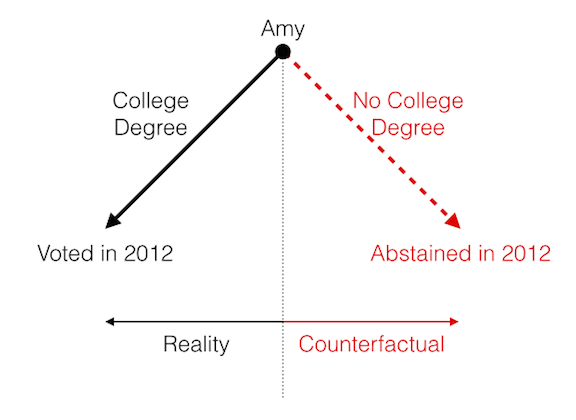
\includegraphics{diagrams/cf-amy.png}
\caption{Effect of education on turning out to vote.}
\end{figure}

\chapter{Literature}\label{literature}

Here is a review of existing methods.

\chapter{Methods}\label{methods}

We describe our methods in this chapter.

\chapter{Applications}\label{applications}

Some \emph{significant} applications are demonstrated in this chapter.

\section{Example one}\label{example-one}

\section{Example two}\label{example-two}

\chapter{Final Words}\label{final-words}

We have finished a nice book.

\bibliography{book.bib,packages.bib}


\end{document}
